\documentclass{article}

% ============================================================
% packages -- superset of everything used across prev_onlines/ and practice/
% ============================================================
\usepackage[T1]{fontenc}      % needed so listings can render a straight " inside code (e.g. f-strings)
\usepackage[top=1in, bottom=1in, left=1in, right=1in]{geometry} % page margins, optional
\usepackage{graphicx}         % \includegraphics
\usepackage{float}            % [H] "put it exactly here" float placement
\usepackage{wrapfig}          % wrapfigure environment (text wraps around image)
\usepackage{caption}
\usepackage{subcaption}       % subfigure environment
\usepackage{booktabs}         % \toprule \midrule \bottomrule (optional cleaner table rules)
\usepackage{array}            % p{}/m{}/b{} paragraph columns, custom column types
\usepackage{enumitem}         % custom list labels/spacing ([label=], itemsep, etc.)
\usepackage[table]{xcolor}    % \textcolor, \rowcolor, \cellcolor
\usepackage{amsmath, amssymb, amsfonts} % core math
\usepackage{amsthm}           % \newtheorem, proof environment
\usepackage{listings}         % code listing, no extra compiler flags needed -- default choice
\usepackage{minted}           % prettier code listing, needs pdflatex -shell-escape + pygments
\usepackage{algorithm}
\usepackage{algpseudocode}    % pseudocode blocks
\usepackage{comment}          % \begin{comment}...\end{comment} to block out text/code
\usepackage[numbers]{natbib}  % \cite, numeric [1] style references
\usepackage{hyperref}         % \href, \url, clickable cross-references
\usepackage{multirow}         % \multirow for tables
\usepackage{minitoc}          % shows up in every solve preamble, rarely actually invoked
\usepackage{authblk}          % multi-author + affiliation blocks

\hypersetup{colorlinks=true, urlcolor=blue, citecolor=black, linkcolor=black}

% minted config -- only takes effect if you compile with: pdflatex -shell-escape
\setminted{
    linenos,
    breaklines,
    frame=single,
    framesep=2mm,
    fontsize=\small,
    bgcolor=gray!5,
    tabsize=4
}

% listings config -- from sir_template.tex (course-taught style), applied to every
% \begin{lstlisting} below by default; no extra compiler flags needed
\definecolor{customblue}{RGB}{0, 76, 153}
\lstset{
    basicstyle=\ttfamily\small,
    keywordstyle=\color{customblue}\bfseries,
    commentstyle=\color{teal!70!black},
    stringstyle=\color{red!70!black},
    frame=single,
    breaklines=true,
    showstringspaces=false,
    columns=fullflexible
}

% custom macros
\newcommand{\set}[1]{\setlength\itemsep{#1em}} % quick list-spacing macro
\newtheorem{proposition}{Proposition}          % needed for the theorem/proof section below

\title{Document Title}
\author{Your Name (Student ID)}
\date{\today}

% ---- multi-author / affiliation alternatives ----
% authblk style, numbered affiliation:
% \author[1]{Author One}
% \affil[1]{Department, University, City}
%
% inline footnote-affiliation style (used in the Laplace solve):
% \author{
% Author A$^{1}$, Author B$^{2}$\\[6pt]
% \small $^{1}$Affiliation A, City\\
% \small $^{2}$Affiliation B, City
% }

\begin{document}

\maketitle
% \tableofcontents \newpage % use only when the article explicitly shows a ToC

\section{Text Formatting}

This sentence has \textbf{bold text}, \textit{italic text}, \emph{emphasized text},
and \underline{underlined text}. \textsc{Small caps} and \texttt{typewriter} also
show up occasionally.

Font sizes: {\small small}, {\normalsize normal}, {\large large}, {\Large Large},
{\LARGE LARGE}, {\huge huge}, {\Huge Huge}.

\textcolor{red}{Colored text in red} and \textcolor{blue}{colored text in blue}
are common for highlighting contrasted statements.

\section{Lists}

\begin{itemize}
    \item Primary item
    \item Secondary item
        \begin{enumerate}
            \item Nested numbered item
            \item[(a)] Custom-labeled sub-item \\ % [(a)] overrides the auto-number for one item
            \item[-] Dash-labeled item
                \begin{itemize}
                    \item[$\dagger$] Symbol-labeled item (dagger)
                    \item[$\diamond$] Symbol-labeled item (diamond)
                    \item[$\rhd$] Symbol-labeled item (triangle)
                \end{itemize}
        \end{enumerate}
\end{itemize}

% custom-lettered / roman-numbered enumerate, and tighter item spacing
\begin{enumerate}[label={(\Roman*)}]
    \item Roman-numbered item
    \item Another roman-numbered item
\end{enumerate}

\begin{enumerate}[leftmargin=*,label=]
    \set{0.5} % \set{n} from the macro above -> \setlength\itemsep{n em}
    \item \textbf{Bold-run-in label} description text continues on the same line;\\
        a manual line break is used above to keep the next line indented under it.
\end{enumerate}

\section{Math}

Inline math uses \verb|$...$|; display math uses \verb|$$...$$|, \verb|\[...\]|,
or the numbered \verb|equation| environment.

Superscripts/subscripts: $x^2$, $x_i$, $x_{i_2}$ (always brace nested subscripts).
Greek: $\alpha, \beta, \gamma, \delta, \pi, \Pi, \sigma, \theta, \omega$.
Fractions: $\frac{a}{b}$ vs.\ $\dfrac{a}{b}$ (display-style, taller); inline
$\displaystyle\frac{a}{b}$ forces the same taller look mid-paragraph.
Roots: $\sqrt{2x+1}$, $\sqrt[5]{2x+1}$.
Sized brackets: $\left(\dfrac{1}{x^2+1}\right)$, $\left[\cdot\right]$,
$\left\{\cdot\right\}$, $\left|\cdot\right|$, one-sided: $\left.\dfrac{dy}{dx}\right|_{x=1}$.
Sums/limits/integrals: $\sum_{i=1}^{n} x_i$, $\lim\limits_{x \to a} f(x)$,
$\int_{0}^{\infty} e^{-st} f(t)\,dt$.
Sets/logic: $\mathbb{R}, \mathbb{Z}, \mathbb{Q}, \mathbb{N}$, $\forall a \in \mathbb{R}$,
$\exists$.

\begin{equation}
    L = I_{ij} \cdot \cos(\theta) + R^2 \label{eq:sample}
\end{equation}

% multi-line derivation that stays inside ONE equation number
\begin{equation}
\begin{split}
    f(x) &= x^2 + 2x + 1 \\
         &= (x+1)^2
\end{split}
\end{equation}

% multi-line derivation where EACH line gets its own number, aligned at &
\begin{align}
    x^2 + 4 &= 4x \\
    (x-2)^2 &= 0 \\
    x &= 2
\end{align}

% piecewise function
\[
p(t) = \begin{cases}
    0, & t < 0, \\
    e^{-t}, & 0 \le t < 3, \\
    \ln(t-2), & t \ge 3
\end{cases}
\]

Equation~\eqref{eq:sample} and Equation~\ref{eq:sample} are the \verb|\eqref|
and \verb|\ref| forms respectively -- \verb|\eqref| auto-adds the parentheses.

\section{Tables}

% plain grid table
\begin{table}[H]
    \centering
    \begin{tabular}{|c|c|c|}
        \hline
        Method & Accuracy & Time Complexity \\
        \hline
        Rasterization & Medium & $O(n)$ \\
        \hline
        Ray Tracing & High & $O(n^2)$ \\
        \hline
    \end{tabular}
    \caption{Plain bordered table}
    \label{tab:plain}
\end{table}

% the tricky combo: multirow + multicolumn + partial \cline rules
\begin{table}[H]
    \centering
    \renewcommand{\arraystretch}{1.5} % taller rows, useful with fractions/multirow
    \begin{tabular}{|c|c|c|c|}
        \hline
        \multirow{2}{*}{\textbf{Family}} & \multicolumn{2}{c|}{\textbf{Equation}} & \multirow{2}{*}{\textbf{Condition}} \\
        \cline{2-3}
        & Time function & Transform & \\
        \hline
        \multirow{2}{*}{Algebraic} & $1$ & $\dfrac{1}{s}$ & $s>0$ \\
        \cline{2-4}
        & $t$ & $\dfrac{1}{s^2}$ & $s>0$ \\
        \hline
    \end{tabular}
    \caption{Multirow + multicolumn table with partial cline rules}
    \label{tab:multi}
\end{table}

% colored table -- header row fill + a paragraph-text column
\begin{table}[H]
    \centering
    \begin{tabular}{|l|p{5cm}|}
        \hline
        \rowcolor{gray!25}
        \textbf{Term} & \textbf{Description} \\
        \hline
        $f(x)$ & \cellcolor{blue!10} A long description that needs to wrap onto
        multiple lines, hence the \texttt{p\{5cm\}} column type instead of \texttt{c}. \\
        \hline
    \end{tabular}
    \caption{Colored table using xcolor[table] (\texttt{rowcolor}/\texttt{cellcolor})}
    \label{tab:colored}
\end{table}

\section{Figures}

% single centered figure
\begin{figure}[H]
    \centering
    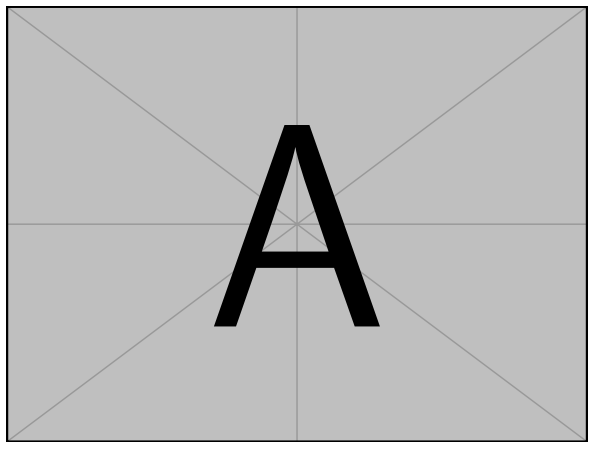
\includegraphics[width=0.4\linewidth]{prev_onlines/22_A2/A.PNG}
    \caption{A single figure}
    \label{fig:single}
\end{figure}

% row of subfigures, side by side
\begin{figure}[H]
    \centering
    \begin{subfigure}{0.3\textwidth}
        \centering
        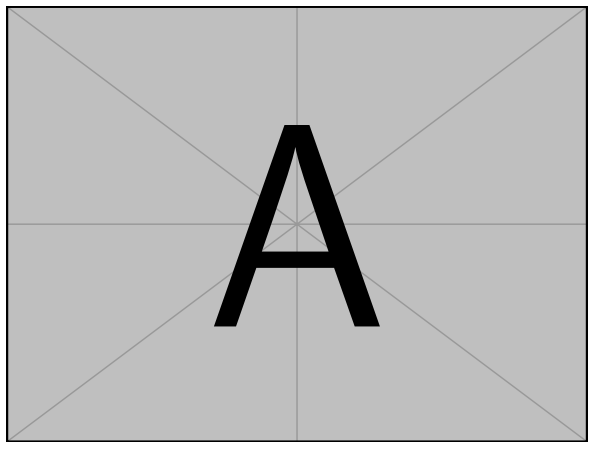
\includegraphics[width=\linewidth]{prev_onlines/22_A2/A.PNG}
        \caption{Output A}
        \label{fig:sub-a}
    \end{subfigure}
    \hfill
    \begin{subfigure}{0.3\textwidth}
        \centering
        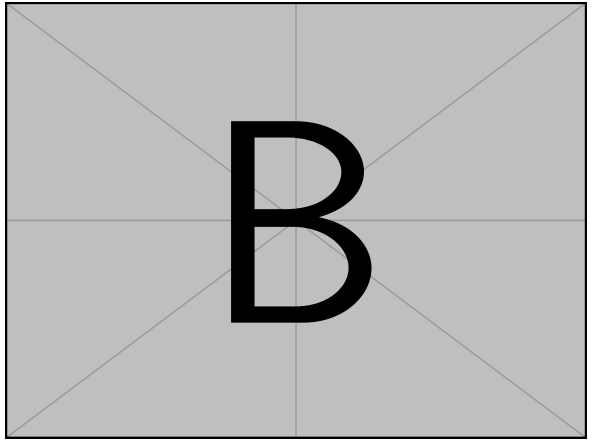
\includegraphics[width=\linewidth]{prev_onlines/22_A2/B.PNG}
        \caption{Output B}
        \label{fig:sub-b}
    \end{subfigure}
    \hfill
    \begin{subfigure}{0.3\textwidth}
        \centering
        
\includegraphics[width=\linewidth]{prev_onlines/22_A2/C.PNG}
        \caption{Output C}
        \label{fig:sub-c}
    \end{subfigure}
    \caption{Three subfigures in a single row, each with its own sub-caption}
    \label{fig:row}
\end{figure}

% asymmetric layout: one dominant subfigure on top, two smaller ones below
\begin{figure}[H]
    \centering
    \begin{subfigure}{0.6\textwidth}
        \centering
        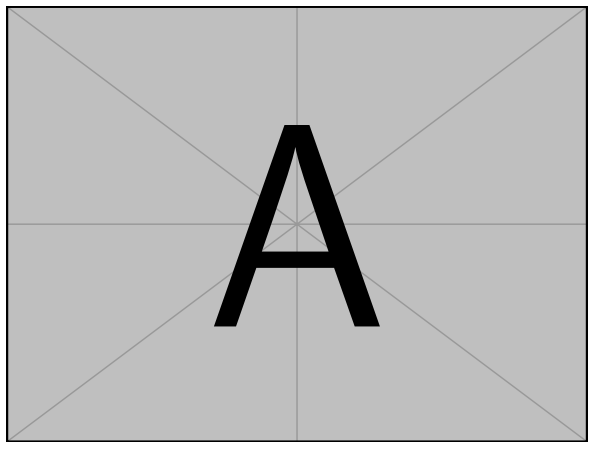
\includegraphics[width=\linewidth]{prev_onlines/22_A2/A.PNG}
        \caption{Main diagram}
        \label{fig:asym-main}
    \end{subfigure}
    \par\medskip
    \begin{subfigure}{0.3\textwidth}
        \centering
        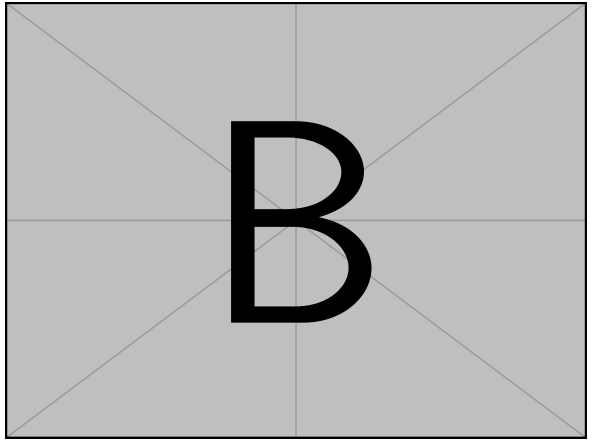
\includegraphics[width=\linewidth]{prev_onlines/22_A2/B.PNG}
        \caption{Detail B}
        \label{fig:asym-b}
    \end{subfigure}
    \hfill
    \begin{subfigure}{0.3\textwidth}
        \centering
        
\includegraphics[width=\linewidth]{prev_onlines/22_A2/C.PNG}
        \caption{Detail C}
        \label{fig:asym-c}
    \end{subfigure}
    \caption{Asymmetric layout: one dominant figure above two smaller ones}
    \label{fig:asym}
\end{figure}

% grid of subfigures with bold row-group labels above each row (e.g. solar system style)
\begin{figure}[H]
    \centering
    \textbf{Row Label One}\par\medskip
    \begin{subfigure}{0.2\textwidth}
        \centering
        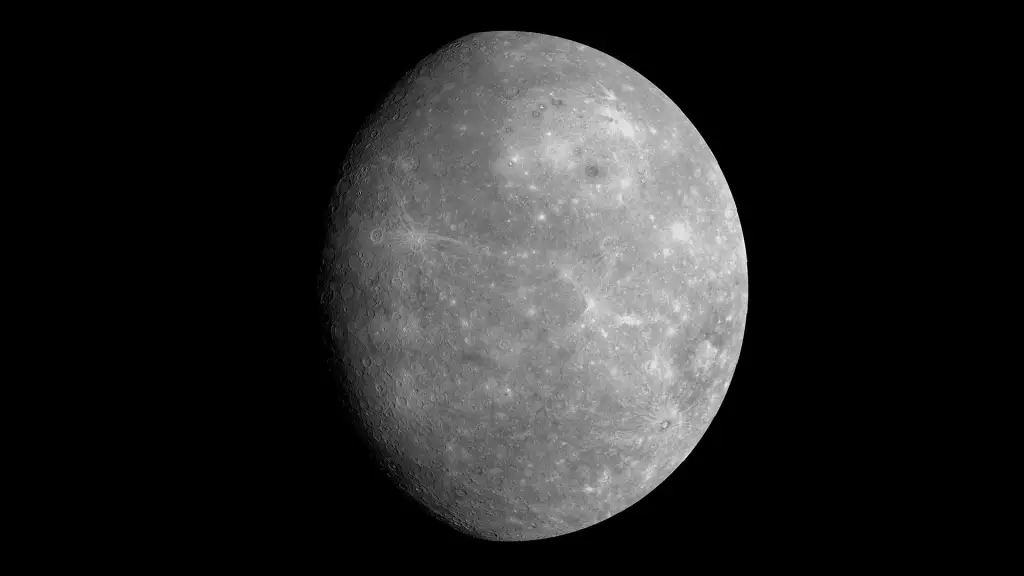
\includegraphics[width=\linewidth]{prev_onlines/23_C2/mercury.png}
        \caption{Mercury}
        \label{fig:grid-mercury}
    \end{subfigure}
    \hfill
    \begin{subfigure}{0.2\textwidth}
        \centering
        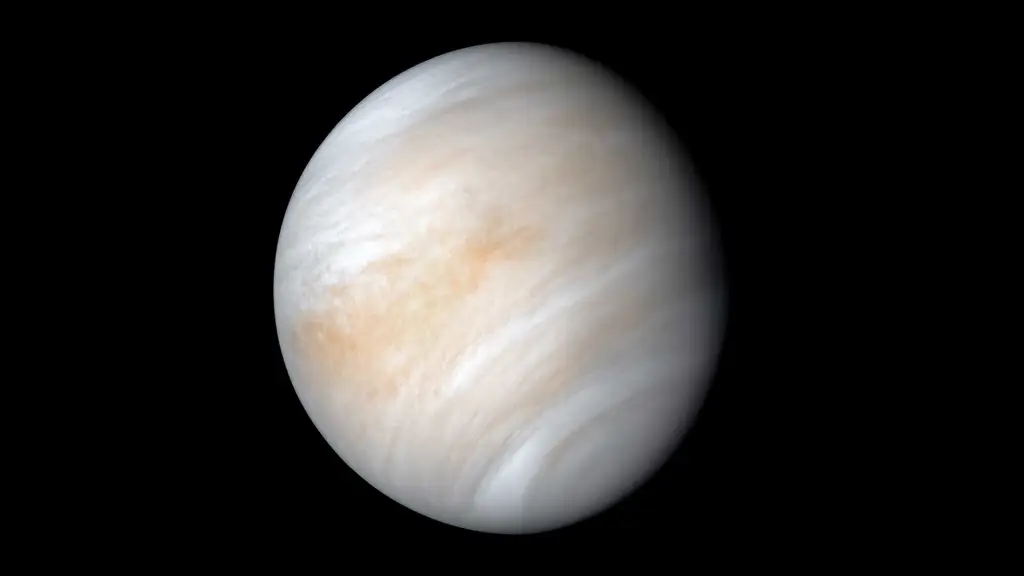
\includegraphics[width=\linewidth]{prev_onlines/23_C2/venus.png}
        \caption{Venus}
        \label{fig:grid-venus}
    \end{subfigure}
    \par\medskip
    \vspace{0.5cm}
    \textbf{Row Label Two}\par\medskip
    \begin{subfigure}{0.2\textwidth}
        \centering
        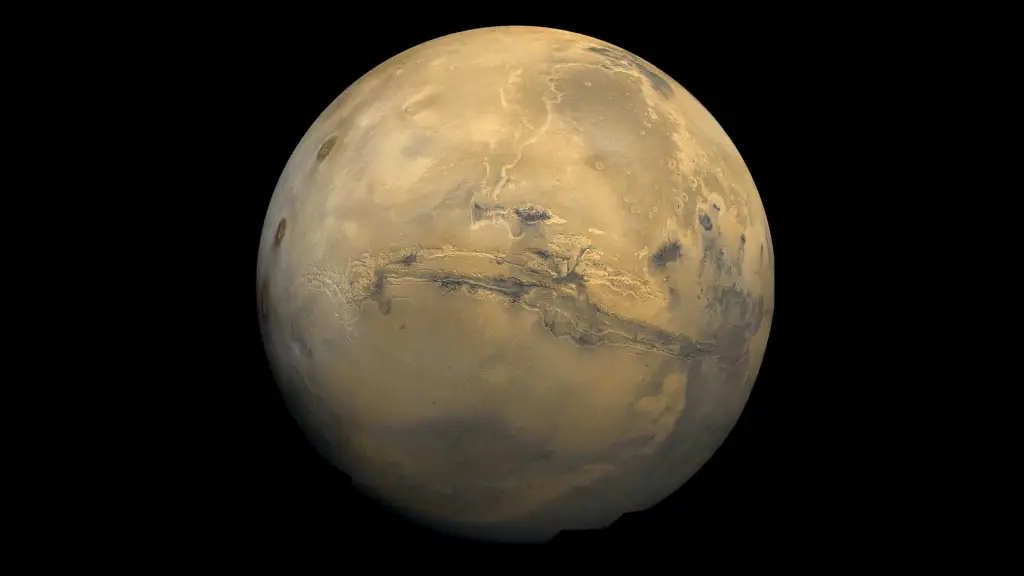
\includegraphics[width=\linewidth]{prev_onlines/23_C2/mars.png}
        \caption{Mars}
        \label{fig:grid-mars}
    \end{subfigure}
    \hfill
    \begin{subfigure}{0.2\textwidth}
        \centering
        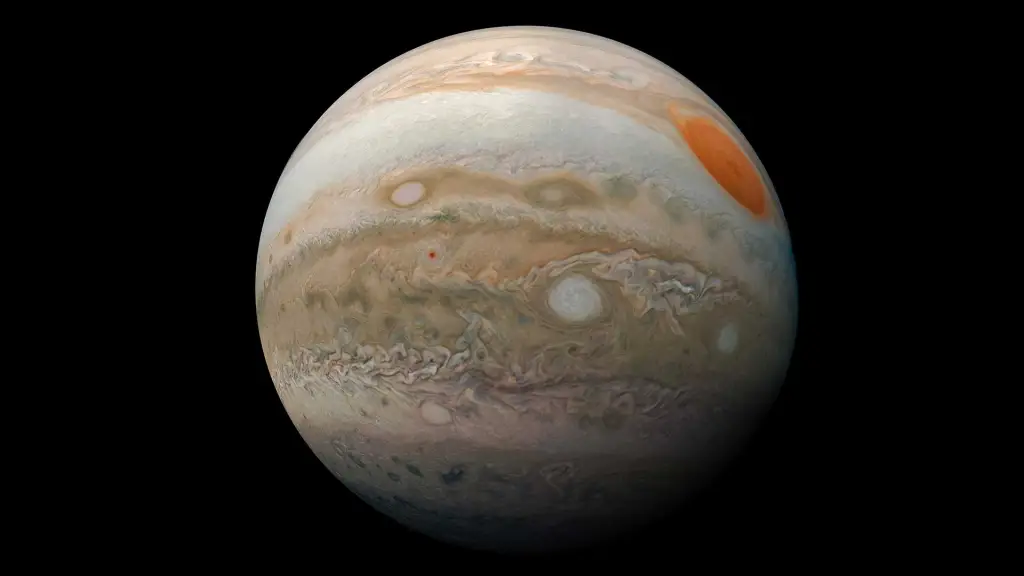
\includegraphics[width=\linewidth]{prev_onlines/23_C2/jupiter.png}
        \caption{Jupiter}
        \label{fig:grid-jupiter}
    \end{subfigure}
    \caption{Grid of subfigures split into labeled row-groups}
    \label{fig:grid}
\end{figure}

% wrapfigure -- image on one side, text wraps around it
\begin{wrapfigure}{r}{0.4\textwidth}
    \centering
    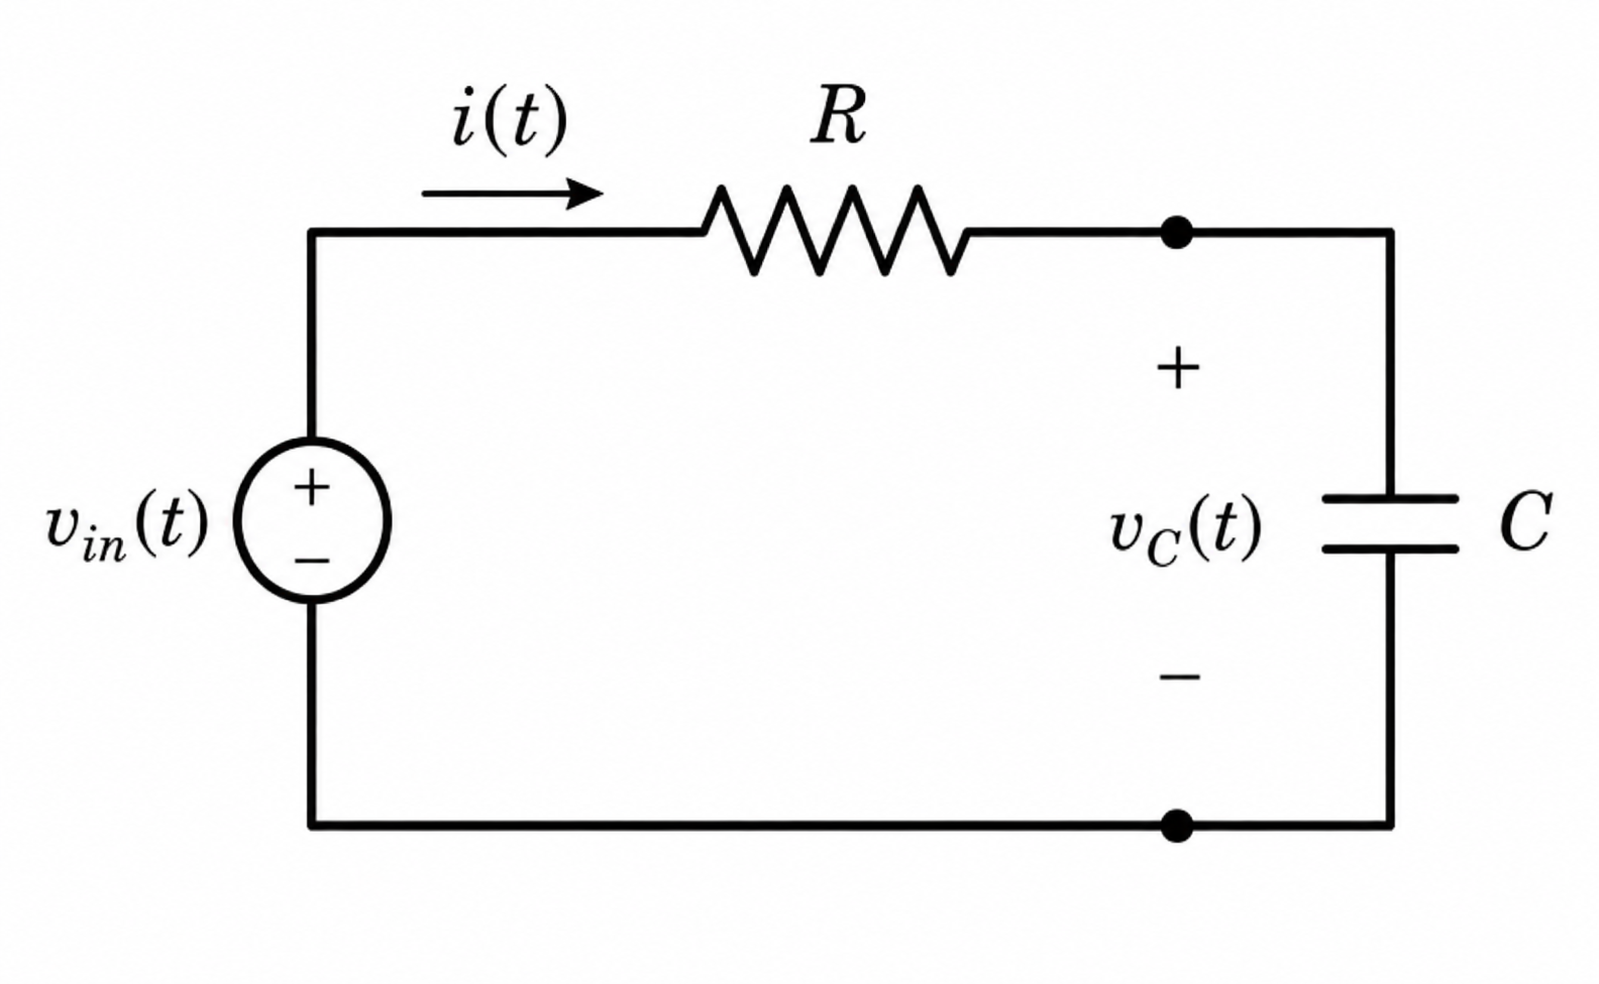
\includegraphics[width=0.38\textwidth]{prev_onlines/23_B1/rc_circuit.png}
    \caption{Wrapped figure}
    \label{fig:wrap}
\end{wrapfigure}
Text placed after a \texttt{wrapfigure} environment flows around the image
instead of stacking above/below it, which is the key visual difference from a
plain \texttt{figure}. Use \texttt{\{r\}} or \texttt{\{l\}} for the side, and a
width fraction for how much horizontal space the wrap reserves. Keep enough
body text below the environment to fill the wrapped height, otherwise later
content can overlap the image.

\clearpage
\section{Code Listings}

% ---- listings: default choice, taught in sir_template.tex -- compiles normally, no shell-escape ----
\begin{lstlisting}[language=Python, caption={A small Python function.}, label={lst:python-square}]
def greet_user(name):
    # Create a greeting message using an f-string
    message = f"Hello, {name}! Welcome to Python."

    # Print the greeting message
    print(message)

    # Return the message in case it's needed elsewhere
    return message


# Example usage
user_name = "Alice"
greet_user(user_name)
\end{lstlisting}

% to pull code from an external file instead of inlining it (as 23_B1 does with rc_response.py):
% \lstinputlisting[language=Python, caption={...}, label={...}]{rc_response.py}

% ---- minted: nicer highlighting, but needs `pdflatex -shell-escape` + pygments --
% sir_template.tex explicitly advises against this in an intro/exam setting unless
% shell-escape is confirmed available; wrapped in \begin{comment} so the file compiles
% by default without it -- delete the comment wrapper (and keep \usepackage{minted} above)
% once shell-escape is confirmed available
\begin{comment}
\begin{listing}[H]
\begin{minted}{python}
from math import exp

def rc_response(resistance, capacitance, input_voltage, times):
    tau = resistance * capacitance
    return [input_voltage * (1 - exp(-t / tau)) for t in times]
\end{minted}
\caption{RC step response (minted package)}
\label{lst:rc-minted}
\end{listing}
\end{comment}

\section{Footnotes, Hyperlinks \& Citations}

A footnote can be attached to any word.\footnote{This is a footnote.}
A raw link: \url{https://www.overleaf.com}. A labeled link:
\href{https://www.overleaf.com}{Overleaf}.

Citations use natbib: \cite{sample2024}. This resolves to a real number (not
\texttt{[?]}) because of the \texttt{thebibliography} block near the end of
this file -- run pdflatex \emph{twice} (or use latexmk) so the \texttt{.aux}
data from the first pass is available to resolve it on the second.

In your actual solves, the bibliography instead comes from an external
\texttt{.bib} file via \verb|\bibliographystyle{...}| + \verb|\bibliography{filename}|
(no \texttt{.bib} extension), which needs a bibtex/biber run in addition to
pdflatex, e.g.\ a file named \texttt{refs.bib} containing:
\begin{verbatim}
@book{sample2024,
    author    = {Author Name},
    title     = {Book Title},
    publisher = {Publisher},
    year      = {2024}
}
\end{verbatim}
Common styles: \texttt{plain}, \texttt{ieeetr}, \texttt{unsrtnat}, \texttt{apalike}.

\section{Theorem and Proof}

\begin{proposition}[Sample proposition]
\label{prop:sample}
For a circular orbit of radius $r$, $\left(\dfrac{v}{c}\right)^2 = \dfrac{GM}{rc^2}$.
\end{proposition}

\begin{proof}
The circular-orbit balance $v^2/r = GM/r^2$ gives $v^2 = GM/r$; divide by $c^2$.
\end{proof}

See Proposition~\ref{prop:sample} for the cross-reference form of a theorem.

% self-contained stand-in for \bibliographystyle+\bibliography+.bib so \cite{sample2024}
% above actually resolves without needing an external .bib file or a bibtex/biber run
\begin{thebibliography}{9}
\bibitem{sample2024} Author Name. \textit{Book Title}. Publisher, 2024.
\end{thebibliography}

\bibliographystyle{unsrtnat}
\bibliography{bib_file_name}

\end{document}
